\documentclass[11pt]{article}
\usepackage[utf8]{inputenc} % Para caracteres en espa�ol
\usepackage{amsmath,amsthm,amsfonts,amssymb,amscd}
\usepackage{multirow,booktabs}
\usepackage[table]{xcolor}
\usepackage{fullpage}
\usepackage{lastpage}
\usepackage{enumitem}
\usepackage{multicol}
\usepackage{fancyhdr}
\usepackage{mathrsfs}
\usepackage{wrapfig}
\usepackage[final]{pdfpages}
\usepackage{setspace}
\usepackage{esvect}
\usepackage{calc}
\usepackage{multicol}
\usepackage{cancel}
\usepackage{graphicx}
\graphicspath{ {pictures/} }
\usepackage[retainorgcmds]{IEEEtrantools}
\usepackage[margin=3cm]{geometry}
\usepackage{amsmath}
\newlength{\tabcont}
\setlength{\parindent}{0.0in}
\setlength{\parskip}{0.05in}
\usepackage{empheq}
\usepackage{framed}
%\usepackage{newtxmath}
\usepackage{euscript}
\DeclareMathAlphabet{\mathpzc}{T1}{pzc}{m}{it}
\usepackage[most]{tcolorbox}
\usepackage{xcolor}
\colorlet{shadecolor}{orange!15}
\parindent 0in
\parskip 12pt
\geometry{margin=1in, headsep=0.25in}
\theoremstyle{definition}
\newtheorem{defn}{Definition}
\newtheorem{reg}{Rule}
\newtheorem{exer}{Exercise}
\newtheorem{note}{Note}
\newcommand{\volume}{{\ooalign{\hfil$V$\hfil\cr\kern0.08em--\hfil\cr}}}
\newcommand{\parr}{\mathbin{\|}} % Parralel Symbol
\begin{document}
\setcounter{section}{3}%Section we want -1
\setcounter{page}{34} %Page we want
\setcounter{equation}{36}%Equation we want -1
\def\thepart{\arabic{part}}
\setcounter{part}{8}
\numberwithin{equation}{part}

 \pagestyle{fancy}
\fancyhf{}
\rhead{Section 8:  Electromagnetic Propulsion - Coaxial Applied-Field Thruster}
\rfoot{Page \thepage}
\thispagestyle{empty}

\begin{center}
{\LARGE \bf Section 8:  Electromagnetic Propulsion}\\
{\large AE435}\\
Spring 2018
\end{center}
\vspace{5mm}
\section{Coaxial Applied-Field Thruster}
\vspace{25mm}
\tableofcontents
\newpage



The physical layout is the same as in a coaxial self-field MPDT, but now you wrap a solenoid around the thruster:

 \begin{center}
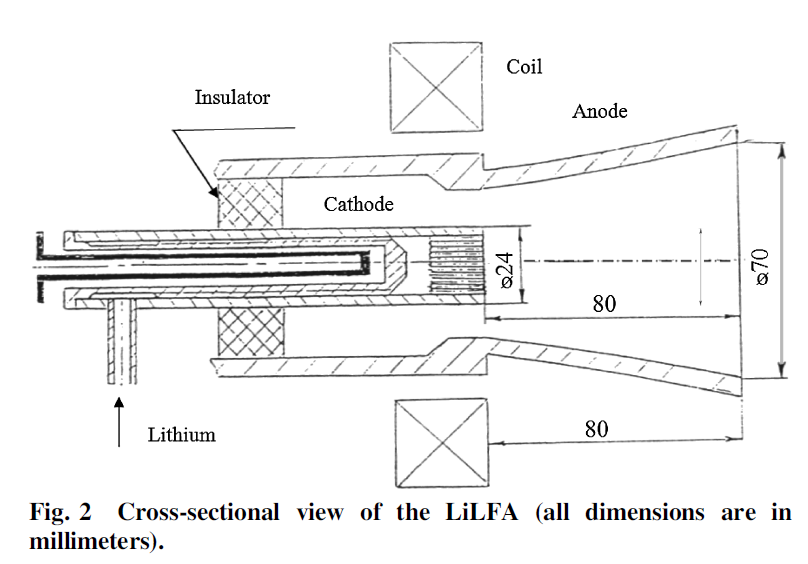
\includegraphics[scale=0.6]{15.png} 
\end{center}

Lev, Choueiri, Propulsion and Power, Vol. 28, No. 3, 2012.
Schematic of the LiLFA (lithium Lorentz force accelerator), initial designed and built by the Moscow Aviation Institute 1998.
\textbf{Specs:}
\begin{itemize}
\item Power: 123-186 kW
\item I$_{sp}$  2760-4240 sec
\item $B_z$  450-900 Gauss
\item Efficiency 35-50$\%$
 \end{itemize}
Applied field increases performance at "low power", power levels less than 100 kW, where self-field is too weak to be effective.
 
Cathode in the LiLFA uses a multichannel hollow cathode

Advantage is a larger cathode surface area, reducing the required current density and thus (by Richardson-Dushman Eqn. 7.72) cathode temperature - provides longer life.
 
An applied axial magnetic field gives rise now to an azimuthal ExB drift.   Since B decreases with axial direction, this swirl motion is converted into axial motion as the jet propagates downstream.  This diverging axial field in the applied-field MPDT can be considered as a \textbf{magnetic nozzle}.

 \begin{center}
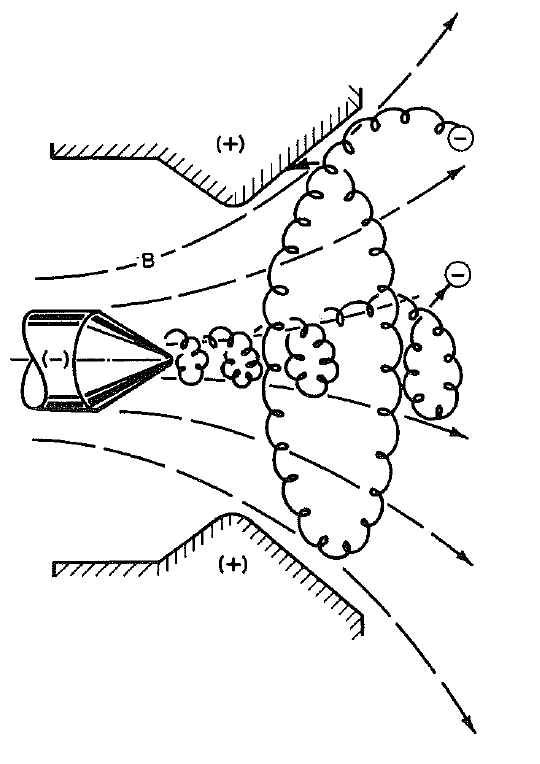
\includegraphics[scale=0.6]{16.png} 
\end{center}

Recent attempts to predict applied-field MPDT performance have only been partially successful.  Best method is still to build and test.  MAI and Princeton have been leaders in this, with work also at NASA Marshall.
\newpage
\subsection{Magnetic Nozzle}

One way to look at the applied-field MPDT is to consider the diverging axial magnetic field as a magnetic nozzle.  Magnetic nozzle also important in other Electrothermal propulsion systems, e.g., helicon, VASIMR, electron-cyclotron resonance (ECR) thrusers
 
Consider the axisymmetric magnetic field from a finite solenoid:
 
 \begin{center}
 \vspace{50mm}
 \textbf{Figure 5: Magnetic Nozzle}
 \end{center}
 
By symmetry
 
\begin{equation*}
\begin{aligned}
B_{\theta} = 0 \\ \\
\frac{\partial \vv{B}}{\partial \theta} = 0
\end{aligned}
\end{equation*}
 
 
To find $B_r$ near the centerline, we use the monopole law:
 
 \begin{equation*}
\begin{aligned}
\nabla \cdot \vv{B} = 0
\end{aligned}
\end{equation*}
 
which  in axisymmetric cylindrical coordinates is:
 
 \begin{equation*}
\begin{aligned}
\frac{1}{r} \, \frac{\partial}{\partial r} (r \, B_r) + \frac{\mathrm{d}B_z}{\mathrm{d}z} = 0
\end{aligned}
\end{equation*}
 
If
\begin{itemize}
\item We know $\frac{\mathrm{d}B_z}{\mathrm{d}z}$ along the centerline (r = 0), and
\item $B_z$ is not a strong function of r,
\end{itemize}
we find that:
 
 \begin{equation*}
\begin{aligned}
r \, B_r = - \int_0^r \, r' \, \frac{\mathrm{d}B_z}{\mathrm{d}z} \, \mathrm{d}r'
\end{aligned}
\end{equation*}
 
where we can pull $\frac{\mathrm{d}B_z}{\mathrm{d}z}$ out of the integral, because not a strong function of r.
 
Which then becomes:
 
 \begin{equation}
\begin{aligned}
r \, B_r \cong -\frac{\mathrm{d}B_z}{\mathrm{d}z} \, \int_0^r \, r' \, \mathrm{d}r'
\end{aligned}
\end{equation}

 \begin{equation*}
\begin{aligned}
r \, B_r = -\frac{1}{2} \, r^2 \, \bigg[\frac{\mathrm{d}B_z}{\mathrm{d}z} \bigg]_{r=0}
\end{aligned}
\end{equation*}
 
so that:
 
 \begin{equation}
\begin{aligned}
B_r = -\frac{1}{2} \, r \, \bigg[\frac{\mathrm{d}B_z}{\mathrm{d}z} \bigg]_{r=0}
\end{aligned}
\end{equation}
 
 
Before we continue, we need to review the \textbf{grad-B drift} (eqn. 3.21).  A gradient in the magnitude of B causes a gradient in the Larmor radius (large at low B, small at high B).  The resulting drift              	is:
\vspace{-5mm}
       	\begin{itemize}
  \item $\perp \, \vv{B}$
  \item $\perp \, \nabla \vv{B}$     	
\item In opposite directions for ions and electrons
 \end{itemize}
Formally, (3.21)
 \begin{equation}
\begin{aligned}
\vv{V}_{\nabla B} = \pm \frac{1}{2} \, v_{\perp} \, r_L \frac{\vv{B} \times \nabla B}{B^2}
\end{aligned}
\end{equation}
 
where the $\pm$ signifies that the direction depends on the charge sign. Top sign, (+), is for Ion. Bottom sign, (-), is for electron. 
 
For the magnetic nozzle:
\vspace{-5mm}
\begin{itemize}
\item $\vv{B}$ is primarily axial
\item   $\nabla B$      	is primarily radial, so
\item  $\vv{V}_{\nabla B}$          	is primarily azimuthal
\end{itemize}
In particular, since              $\frac{\partial \vv{B}}{\partial \theta} = 0$,             there is no radial component to the grad-B drift.
 
If we consider the Lorentz force terms in this magnetic field:
 
 \begin{equation*}
\begin{aligned}
F_r &= q \, (v_{\theta}\,B_z - v_z \, B_{\theta}) \\ \\
F_{\theta} &= q \, (-v_{r}\,B_z + v_z \, B_r) \\ \\
F_z &= q \, (v_r\,B_{\theta} - v_{\theta} \, B_{r})
\end{aligned}
\end{equation*}
\vspace{-5mm}
\begin{itemize} 
\item Terms with      $B_{\theta}$  	cancel out
\item Terms with      $v_{\theta}$ and $v_r$   	are simply the usual Larmor gyration (1) and (2)
\item Term 3 vanishes on $r = 0$, where $B_r =0$.  Off the centerline this term causes a radial drift along B, as the nozzle expands this helps particles slip off the Bfield lines.
\item Term 4 creates an axial force (thrust)
\begin{equation}
\begin{aligned}
F_z = \frac{1}{2} \, q \, v_{\theta} \, r \, \bigg[\frac{\mathrm{d}B_z}{\mathrm{d}z} \bigg]
\end{aligned}
\end{equation}
 \end{itemize}
 
 
Consider a particle rotating about the axis at r =rL with constant gyrospeed:
\begin{equation*}
\begin{aligned}
v_{\theta} = \mp v_{\perp}
\end{aligned}
\end{equation*}
 
\textbf{Why did the signs flip?} The ions are now negative and the electrons are now positive. This is because they orbit so as to oppose the applied magnetic field.  

The average force on this particle over a gyration is
 
 \begin{equation*}
\begin{aligned}
F_z = \mp \, q \, v_{\perp} \, r_L \, \frac{\mathrm{d}B_z}{\mathrm{d}z}
\end{aligned}
\end{equation*}
 
with the Larmor radius (3.11) and gyrofrequency (3.8), this becomes:
 
 \begin{equation}
\begin{aligned}
F_z = - \frac{1}{2} \, \frac{m \, v_{\perp}^2}{B} \, \frac{\mathrm{d}B_z}{\mathrm{d}z}
\end{aligned}
\end{equation}
 
We can define the \textbf{magnetic moment} of the gyrating particle as:

 \begin{equation}
\begin{aligned}
\mu_B = \frac{1}{2} \, \frac{m \, v_{\perp}^2}{B}
\end{aligned}
\end{equation}
 \newpage
such that

 \begin{equation}
\begin{aligned}
F_z = - \mu_B \, \frac{\mathrm{d}B_z}{\mathrm{d}z}
\end{aligned}
\end{equation}
 
One can show that     $\mu_B$  	is:
\begin{enumerate}
\item The \textbf{magnetic dipole moment} $\mu_B=J \, \oint \, \vv{r} \times \mathrm{d}\vv{l} $                      	of the current loop defined by the gyrating charge. We can think of the charged particles motion as a current loop and they move so as to conserve that magnetic flux within their gyro orbit. Not just for their gyro motion but also for their drifting. 
\item \textbf{Invariant} , i.e., not changing with B.

This means that as the charge particle moves from the throat (strong B) to the exit (weak B),     $v_{\perp}$      must decrease to keep      $\mu_B$    constant.

Since a steady magnetic field can do no work,       $v_{||}$ 	must increase (conservation of energy!).

 \begin{equation*}
\begin{aligned}
v_{tot}^2 = v_{\perp}^{2} + v_{||}^2
\end{aligned}
\end{equation*}
 \end{enumerate}
 
So, we're converting intense azimuthal kinetic energy (or "swirl") in the throat to intense axial kinetic energy at the exit.
 
 Two cases:
 \vspace{-5mm}
 \begin{itemize}
\item For a single solenoid, we have a magnetic nozzle
\item For two coaxial solenoids, we have a magnetic bottle or magnetic mirror.
\end{itemize}
Magnetic mirrors (bottles) were one of the earliest methods attempted for controlled fusion reactions.  It turns out they are prone to end-cone losses (when          $\frac{v_{||}}{v_{\perp}}$ 	at the plane of axial symmetry is too high to be reflected) and macro instabilities (Rayleigh-Taylor), as well as micro-instabilities (velocity distribution depletion by end-cone losses).
\end{document}